\documentclass[border=5pt]{standalone}
\usepackage[T1]{fontenc}\usepackage{lmodern}\usepackage{pgfplots}
\pgfplotsset{compat=1.18}\begin{document}\sffamily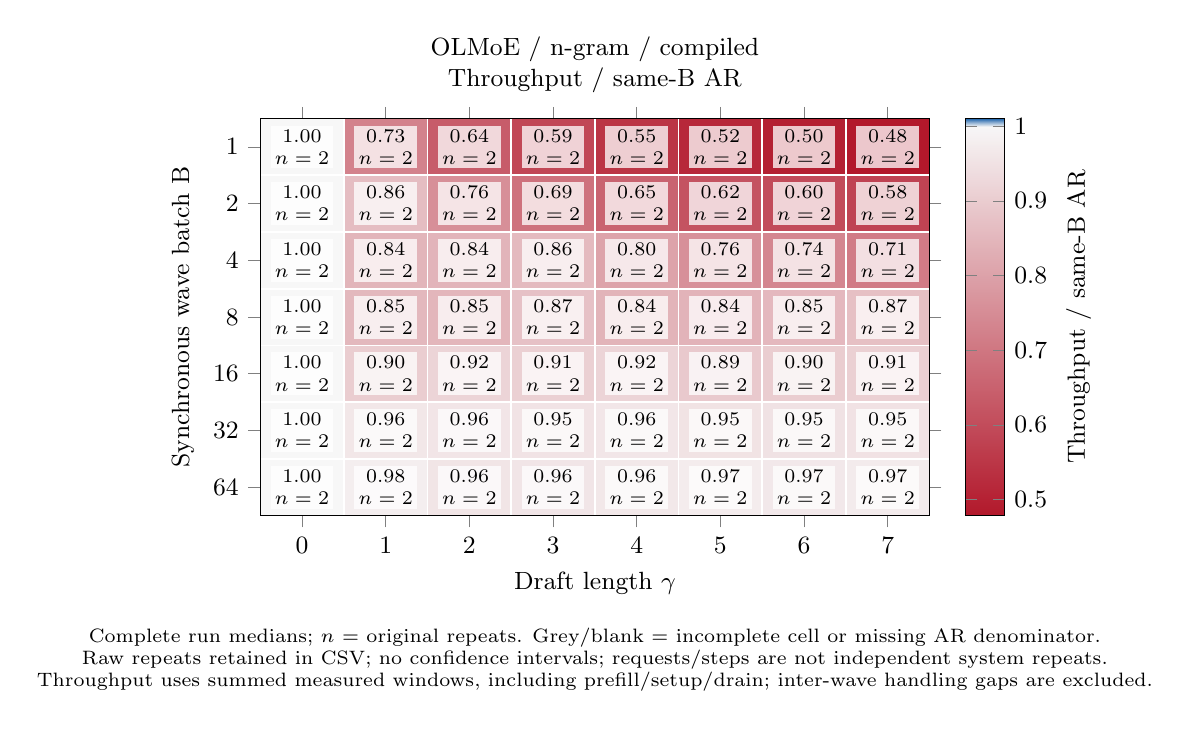
\begin{tikzpicture}
\begin{axis}[name=matrix,width=8.50cm,height=5.04cm,scale only axis,xmin=-.5,xmax=7.5,ymin=-.5,ymax=6.5,y dir=reverse,axis on top,tick align=outside,xtick={0,1,2,3,4,5,6,7},xticklabels={0,1,2,3,4,5,6,7},ytick={0,1,2,3,4,5,6},yticklabels={1,2,4,8,16,32,64},xlabel={Draft length $\gamma$},ylabel={Synchronous wave batch B},title={OLMoE / n-gram / compiled\\Throughput / same-B AR},title style={align=center,font=\small},tick label style={font=\small},label style={font=\small},point meta min=0.478835166381,point meta max=1.01,colormap={matrixcolors}{rgb255=(178,24,43); rgb255=(179,26,45); rgb255=(179,29,47); rgb255=(180,31,49); rgb255=(181,33,51); rgb255=(182,35,53); rgb255=(182,38,55); rgb255=(183,40,58); rgb255=(184,42,60); rgb255=(184,44,62); rgb255=(185,47,64); rgb255=(186,49,66); rgb255=(186,51,68); rgb255=(187,54,70); rgb255=(188,56,72); rgb255=(189,58,74); rgb255=(189,60,76); rgb255=(190,63,78); rgb255=(191,65,80); rgb255=(191,67,83); rgb255=(192,69,85); rgb255=(193,72,87); rgb255=(193,74,89); rgb255=(194,76,91); rgb255=(195,79,93); rgb255=(196,81,95); rgb255=(196,83,97); rgb255=(197,85,99); rgb255=(198,88,101); rgb255=(198,90,103); rgb255=(199,92,105); rgb255=(200,94,107); rgb255=(201,97,110); rgb255=(201,99,112); rgb255=(202,101,114); rgb255=(203,104,116); rgb255=(203,106,118); rgb255=(204,108,120); rgb255=(205,110,122); rgb255=(205,113,124); rgb255=(206,115,126); rgb255=(207,117,128); rgb255=(208,119,130); rgb255=(208,122,132); rgb255=(209,124,134); rgb255=(210,126,137); rgb255=(210,129,139); rgb255=(211,131,141); rgb255=(212,133,143); rgb255=(212,135,145); rgb255=(213,138,147); rgb255=(214,140,149); rgb255=(215,142,151); rgb255=(215,144,153); rgb255=(216,147,155); rgb255=(217,149,157); rgb255=(217,151,159); rgb255=(218,154,162); rgb255=(219,156,164); rgb255=(219,158,166); rgb255=(220,160,168); rgb255=(221,163,170); rgb255=(222,165,172); rgb255=(222,167,174); rgb255=(223,169,176); rgb255=(224,172,178); rgb255=(224,174,180); rgb255=(225,176,182); rgb255=(226,179,184); rgb255=(227,181,186); rgb255=(227,183,189); rgb255=(228,185,191); rgb255=(229,188,193); rgb255=(229,190,195); rgb255=(230,192,197); rgb255=(231,194,199); rgb255=(231,197,201); rgb255=(232,199,203); rgb255=(233,201,205); rgb255=(234,204,207); rgb255=(234,206,209); rgb255=(235,208,211); rgb255=(236,210,213); rgb255=(236,213,216); rgb255=(237,215,218); rgb255=(238,217,220); rgb255=(238,219,222); rgb255=(239,222,224); rgb255=(240,224,226); rgb255=(241,226,228); rgb255=(241,229,230); rgb255=(242,231,232); rgb255=(243,233,234); rgb255=(243,235,236); rgb255=(244,238,238); rgb255=(245,240,241); rgb255=(246,242,243); rgb255=(246,244,245); rgb255=(247,247,247); rgb255=(147,179,212); rgb255=(33,102,172)},colorbar,colorbar style={ylabel={Throughput / same-B AR},label style={font=\small},tick label style={font=\small}}]
\path[fill={rgb,255:red,247;green,247;blue,247},draw=white,line width=.6pt] (axis cs:-0.5,-0.5) rectangle (axis cs:0.5,0.5);
\node[align=center,font=\scriptsize,fill=white,fill opacity=.76,text opacity=1,inner sep=1.5pt] at (axis cs:0,0) {1.00\\$n=2$};
\path[fill={rgb,255:red,211;green,130;blue,140},draw=white,line width=.6pt] (axis cs:0.5,-0.5) rectangle (axis cs:1.5,0.5);
\node[align=center,font=\scriptsize,fill=white,fill opacity=.76,text opacity=1,inner sep=1.5pt] at (axis cs:1,0) {0.73\\$n=2$};
\path[fill={rgb,255:red,199;green,92;blue,106},draw=white,line width=.6pt] (axis cs:1.5,-0.5) rectangle (axis cs:2.5,0.5);
\node[align=center,font=\scriptsize,fill=white,fill opacity=.76,text opacity=1,inner sep=1.5pt] at (axis cs:2,0) {0.64\\$n=2$};
\path[fill={rgb,255:red,193;green,71;blue,86},draw=white,line width=.6pt] (axis cs:2.5,-0.5) rectangle (axis cs:3.5,0.5);
\node[align=center,font=\scriptsize,fill=white,fill opacity=.76,text opacity=1,inner sep=1.5pt] at (axis cs:3,0) {0.59\\$n=2$};
\path[fill={rgb,255:red,187;green,53;blue,69},draw=white,line width=.6pt] (axis cs:3.5,-0.5) rectangle (axis cs:4.5,0.5);
\node[align=center,font=\scriptsize,fill=white,fill opacity=.76,text opacity=1,inner sep=1.5pt] at (axis cs:4,0) {0.55\\$n=2$};
\path[fill={rgb,255:red,183;green,40;blue,58},draw=white,line width=.6pt] (axis cs:4.5,-0.5) rectangle (axis cs:5.5,0.5);
\node[align=center,font=\scriptsize,fill=white,fill opacity=.76,text opacity=1,inner sep=1.5pt] at (axis cs:5,0) {0.52\\$n=2$};
\path[fill={rgb,255:red,180;green,32;blue,50},draw=white,line width=.6pt] (axis cs:5.5,-0.5) rectangle (axis cs:6.5,0.5);
\node[align=center,font=\scriptsize,fill=white,fill opacity=.76,text opacity=1,inner sep=1.5pt] at (axis cs:6,0) {0.50\\$n=2$};
\path[fill={rgb,255:red,178;green,24;blue,43},draw=white,line width=.6pt] (axis cs:6.5,-0.5) rectangle (axis cs:7.5,0.5);
\node[align=center,font=\scriptsize,fill=white,fill opacity=.76,text opacity=1,inner sep=1.5pt] at (axis cs:7,0) {0.48\\$n=2$};
\path[fill={rgb,255:red,247;green,247;blue,247},draw=white,line width=.6pt] (axis cs:-0.5,0.5) rectangle (axis cs:0.5,1.5);
\node[align=center,font=\scriptsize,fill=white,fill opacity=.76,text opacity=1,inner sep=1.5pt] at (axis cs:0,1) {1.00\\$n=2$};
\path[fill={rgb,255:red,229;green,189;blue,194},draw=white,line width=.6pt] (axis cs:0.5,0.5) rectangle (axis cs:1.5,1.5);
\node[align=center,font=\scriptsize,fill=white,fill opacity=.76,text opacity=1,inner sep=1.5pt] at (axis cs:1,1) {0.86\\$n=2$};
\path[fill={rgb,255:red,215;green,143;blue,152},draw=white,line width=.6pt] (axis cs:1.5,0.5) rectangle (axis cs:2.5,1.5);
\node[align=center,font=\scriptsize,fill=white,fill opacity=.76,text opacity=1,inner sep=1.5pt] at (axis cs:2,1) {0.76\\$n=2$};
\path[fill={rgb,255:red,206;green,114;blue,125},draw=white,line width=.6pt] (axis cs:2.5,0.5) rectangle (axis cs:3.5,1.5);
\node[align=center,font=\scriptsize,fill=white,fill opacity=.76,text opacity=1,inner sep=1.5pt] at (axis cs:3,1) {0.69\\$n=2$};
\path[fill={rgb,255:red,201;green,99;blue,112},draw=white,line width=.6pt] (axis cs:3.5,0.5) rectangle (axis cs:4.5,1.5);
\node[align=center,font=\scriptsize,fill=white,fill opacity=.76,text opacity=1,inner sep=1.5pt] at (axis cs:4,1) {0.65\\$n=2$};
\path[fill={rgb,255:red,196;green,83;blue,97},draw=white,line width=.6pt] (axis cs:4.5,0.5) rectangle (axis cs:5.5,1.5);
\node[align=center,font=\scriptsize,fill=white,fill opacity=.76,text opacity=1,inner sep=1.5pt] at (axis cs:5,1) {0.62\\$n=2$};
\path[fill={rgb,255:red,194;green,75;blue,90},draw=white,line width=.6pt] (axis cs:5.5,0.5) rectangle (axis cs:6.5,1.5);
\node[align=center,font=\scriptsize,fill=white,fill opacity=.76,text opacity=1,inner sep=1.5pt] at (axis cs:6,1) {0.60\\$n=2$};
\path[fill={rgb,255:red,191;green,67;blue,83},draw=white,line width=.6pt] (axis cs:6.5,0.5) rectangle (axis cs:7.5,1.5);
\node[align=center,font=\scriptsize,fill=white,fill opacity=.76,text opacity=1,inner sep=1.5pt] at (axis cs:7,1) {0.58\\$n=2$};
\path[fill={rgb,255:red,247;green,247;blue,247},draw=white,line width=.6pt] (axis cs:-0.5,1.5) rectangle (axis cs:0.5,2.5);
\node[align=center,font=\scriptsize,fill=white,fill opacity=.76,text opacity=1,inner sep=1.5pt] at (axis cs:0,2) {1.00\\$n=2$};
\path[fill={rgb,255:red,226;green,181;blue,186},draw=white,line width=.6pt] (axis cs:0.5,1.5) rectangle (axis cs:1.5,2.5);
\node[align=center,font=\scriptsize,fill=white,fill opacity=.76,text opacity=1,inner sep=1.5pt] at (axis cs:1,2) {0.84\\$n=2$};
\path[fill={rgb,255:red,226;green,180;blue,186},draw=white,line width=.6pt] (axis cs:1.5,1.5) rectangle (axis cs:2.5,2.5);
\node[align=center,font=\scriptsize,fill=white,fill opacity=.76,text opacity=1,inner sep=1.5pt] at (axis cs:2,2) {0.84\\$n=2$};
\path[fill={rgb,255:red,228;green,186;blue,191},draw=white,line width=.6pt] (axis cs:2.5,1.5) rectangle (axis cs:3.5,2.5);
\node[align=center,font=\scriptsize,fill=white,fill opacity=.76,text opacity=1,inner sep=1.5pt] at (axis cs:3,2) {0.86\\$n=2$};
\path[fill={rgb,255:red,221;green,163;blue,170},draw=white,line width=.6pt] (axis cs:3.5,1.5) rectangle (axis cs:4.5,2.5);
\node[align=center,font=\scriptsize,fill=white,fill opacity=.76,text opacity=1,inner sep=1.5pt] at (axis cs:4,2) {0.80\\$n=2$};
\path[fill={rgb,255:red,215;green,144;blue,153},draw=white,line width=.6pt] (axis cs:4.5,1.5) rectangle (axis cs:5.5,2.5);
\node[align=center,font=\scriptsize,fill=white,fill opacity=.76,text opacity=1,inner sep=1.5pt] at (axis cs:5,2) {0.76\\$n=2$};
\path[fill={rgb,255:red,212;green,134;blue,144},draw=white,line width=.6pt] (axis cs:5.5,1.5) rectangle (axis cs:6.5,2.5);
\node[align=center,font=\scriptsize,fill=white,fill opacity=.76,text opacity=1,inner sep=1.5pt] at (axis cs:6,2) {0.74\\$n=2$};
\path[fill={rgb,255:red,209;green,123;blue,134},draw=white,line width=.6pt] (axis cs:6.5,1.5) rectangle (axis cs:7.5,2.5);
\node[align=center,font=\scriptsize,fill=white,fill opacity=.76,text opacity=1,inner sep=1.5pt] at (axis cs:7,2) {0.71\\$n=2$};
\path[fill={rgb,255:red,247;green,247;blue,247},draw=white,line width=.6pt] (axis cs:-0.5,2.5) rectangle (axis cs:0.5,3.5);
\node[align=center,font=\scriptsize,fill=white,fill opacity=.76,text opacity=1,inner sep=1.5pt] at (axis cs:0,3) {1.00\\$n=2$};
\path[fill={rgb,255:red,227;green,184;blue,189},draw=white,line width=.6pt] (axis cs:0.5,2.5) rectangle (axis cs:1.5,3.5);
\node[align=center,font=\scriptsize,fill=white,fill opacity=.76,text opacity=1,inner sep=1.5pt] at (axis cs:1,3) {0.85\\$n=2$};
\path[fill={rgb,255:red,227;green,182;blue,187},draw=white,line width=.6pt] (axis cs:1.5,2.5) rectangle (axis cs:2.5,3.5);
\node[align=center,font=\scriptsize,fill=white,fill opacity=.76,text opacity=1,inner sep=1.5pt] at (axis cs:2,3) {0.85\\$n=2$};
\path[fill={rgb,255:red,230;green,193;blue,198},draw=white,line width=.6pt] (axis cs:2.5,2.5) rectangle (axis cs:3.5,3.5);
\node[align=center,font=\scriptsize,fill=white,fill opacity=.76,text opacity=1,inner sep=1.5pt] at (axis cs:3,3) {0.87\\$n=2$};
\path[fill={rgb,255:red,226;green,180;blue,185},draw=white,line width=.6pt] (axis cs:3.5,2.5) rectangle (axis cs:4.5,3.5);
\node[align=center,font=\scriptsize,fill=white,fill opacity=.76,text opacity=1,inner sep=1.5pt] at (axis cs:4,3) {0.84\\$n=2$};
\path[fill={rgb,255:red,226;green,179;blue,185},draw=white,line width=.6pt] (axis cs:4.5,2.5) rectangle (axis cs:5.5,3.5);
\node[align=center,font=\scriptsize,fill=white,fill opacity=.76,text opacity=1,inner sep=1.5pt] at (axis cs:5,3) {0.84\\$n=2$};
\path[fill={rgb,255:red,228;green,184;blue,190},draw=white,line width=.6pt] (axis cs:5.5,2.5) rectangle (axis cs:6.5,3.5);
\node[align=center,font=\scriptsize,fill=white,fill opacity=.76,text opacity=1,inner sep=1.5pt] at (axis cs:6,3) {0.85\\$n=2$};
\path[fill={rgb,255:red,230;green,192;blue,196},draw=white,line width=.6pt] (axis cs:6.5,2.5) rectangle (axis cs:7.5,3.5);
\node[align=center,font=\scriptsize,fill=white,fill opacity=.76,text opacity=1,inner sep=1.5pt] at (axis cs:7,3) {0.87\\$n=2$};
\path[fill={rgb,255:red,247;green,247;blue,247},draw=white,line width=.6pt] (axis cs:-0.5,3.5) rectangle (axis cs:0.5,4.5);
\node[align=center,font=\scriptsize,fill=white,fill opacity=.76,text opacity=1,inner sep=1.5pt] at (axis cs:0,4) {1.00\\$n=2$};
\path[fill={rgb,255:red,234;green,205;blue,208},draw=white,line width=.6pt] (axis cs:0.5,3.5) rectangle (axis cs:1.5,4.5);
\node[align=center,font=\scriptsize,fill=white,fill opacity=.76,text opacity=1,inner sep=1.5pt] at (axis cs:1,4) {0.90\\$n=2$};
\path[fill={rgb,255:red,236;green,212;blue,215},draw=white,line width=.6pt] (axis cs:1.5,3.5) rectangle (axis cs:2.5,4.5);
\node[align=center,font=\scriptsize,fill=white,fill opacity=.76,text opacity=1,inner sep=1.5pt] at (axis cs:2,4) {0.92\\$n=2$};
\path[fill={rgb,255:red,235;green,208;blue,211},draw=white,line width=.6pt] (axis cs:2.5,3.5) rectangle (axis cs:3.5,4.5);
\node[align=center,font=\scriptsize,fill=white,fill opacity=.76,text opacity=1,inner sep=1.5pt] at (axis cs:3,4) {0.91\\$n=2$};
\path[fill={rgb,255:red,236;green,212;blue,215},draw=white,line width=.6pt] (axis cs:3.5,3.5) rectangle (axis cs:4.5,4.5);
\node[align=center,font=\scriptsize,fill=white,fill opacity=.76,text opacity=1,inner sep=1.5pt] at (axis cs:4,4) {0.92\\$n=2$};
\path[fill={rgb,255:red,233;green,201;blue,205},draw=white,line width=.6pt] (axis cs:4.5,3.5) rectangle (axis cs:5.5,4.5);
\node[align=center,font=\scriptsize,fill=white,fill opacity=.76,text opacity=1,inner sep=1.5pt] at (axis cs:5,4) {0.89\\$n=2$};
\path[fill={rgb,255:red,234;green,205;blue,208},draw=white,line width=.6pt] (axis cs:5.5,3.5) rectangle (axis cs:6.5,4.5);
\node[align=center,font=\scriptsize,fill=white,fill opacity=.76,text opacity=1,inner sep=1.5pt] at (axis cs:6,4) {0.90\\$n=2$};
\path[fill={rgb,255:red,235;green,208;blue,211},draw=white,line width=.6pt] (axis cs:6.5,3.5) rectangle (axis cs:7.5,4.5);
\node[align=center,font=\scriptsize,fill=white,fill opacity=.76,text opacity=1,inner sep=1.5pt] at (axis cs:7,4) {0.91\\$n=2$};
\path[fill={rgb,255:red,247;green,247;blue,247},draw=white,line width=.6pt] (axis cs:-0.5,4.5) rectangle (axis cs:0.5,5.5);
\node[align=center,font=\scriptsize,fill=white,fill opacity=.76,text opacity=1,inner sep=1.5pt] at (axis cs:0,5) {1.00\\$n=2$};
\path[fill={rgb,255:red,242;green,231;blue,232},draw=white,line width=.6pt] (axis cs:0.5,4.5) rectangle (axis cs:1.5,5.5);
\node[align=center,font=\scriptsize,fill=white,fill opacity=.76,text opacity=1,inner sep=1.5pt] at (axis cs:1,5) {0.96\\$n=2$};
\path[fill={rgb,255:red,242;green,229;blue,231},draw=white,line width=.6pt] (axis cs:1.5,4.5) rectangle (axis cs:2.5,5.5);
\node[align=center,font=\scriptsize,fill=white,fill opacity=.76,text opacity=1,inner sep=1.5pt] at (axis cs:2,5) {0.96\\$n=2$};
\path[fill={rgb,255:red,241;green,227;blue,229},draw=white,line width=.6pt] (axis cs:2.5,4.5) rectangle (axis cs:3.5,5.5);
\node[align=center,font=\scriptsize,fill=white,fill opacity=.76,text opacity=1,inner sep=1.5pt] at (axis cs:3,5) {0.95\\$n=2$};
\path[fill={rgb,255:red,242;green,230;blue,232},draw=white,line width=.6pt] (axis cs:3.5,4.5) rectangle (axis cs:4.5,5.5);
\node[align=center,font=\scriptsize,fill=white,fill opacity=.76,text opacity=1,inner sep=1.5pt] at (axis cs:4,5) {0.96\\$n=2$};
\path[fill={rgb,255:red,241;green,227;blue,228},draw=white,line width=.6pt] (axis cs:4.5,4.5) rectangle (axis cs:5.5,5.5);
\node[align=center,font=\scriptsize,fill=white,fill opacity=.76,text opacity=1,inner sep=1.5pt] at (axis cs:5,5) {0.95\\$n=2$};
\path[fill={rgb,255:red,240;green,226;blue,228},draw=white,line width=.6pt] (axis cs:5.5,4.5) rectangle (axis cs:6.5,5.5);
\node[align=center,font=\scriptsize,fill=white,fill opacity=.76,text opacity=1,inner sep=1.5pt] at (axis cs:6,5) {0.95\\$n=2$};
\path[fill={rgb,255:red,241;green,226;blue,228},draw=white,line width=.6pt] (axis cs:6.5,4.5) rectangle (axis cs:7.5,5.5);
\node[align=center,font=\scriptsize,fill=white,fill opacity=.76,text opacity=1,inner sep=1.5pt] at (axis cs:7,5) {0.95\\$n=2$};
\path[fill={rgb,255:red,247;green,247;blue,247},draw=white,line width=.6pt] (axis cs:-0.5,5.5) rectangle (axis cs:0.5,6.5);
\node[align=center,font=\scriptsize,fill=white,fill opacity=.76,text opacity=1,inner sep=1.5pt] at (axis cs:0,6) {1.00\\$n=2$};
\path[fill={rgb,255:red,244;green,238;blue,239},draw=white,line width=.6pt] (axis cs:0.5,5.5) rectangle (axis cs:1.5,6.5);
\node[align=center,font=\scriptsize,fill=white,fill opacity=.76,text opacity=1,inner sep=1.5pt] at (axis cs:1,6) {0.98\\$n=2$};
\path[fill={rgb,255:red,241;green,229;blue,230},draw=white,line width=.6pt] (axis cs:1.5,5.5) rectangle (axis cs:2.5,6.5);
\node[align=center,font=\scriptsize,fill=white,fill opacity=.76,text opacity=1,inner sep=1.5pt] at (axis cs:2,6) {0.96\\$n=2$};
\path[fill={rgb,255:red,241;green,229;blue,231},draw=white,line width=.6pt] (axis cs:2.5,5.5) rectangle (axis cs:3.5,6.5);
\node[align=center,font=\scriptsize,fill=white,fill opacity=.76,text opacity=1,inner sep=1.5pt] at (axis cs:3,6) {0.96\\$n=2$};
\path[fill={rgb,255:red,242;green,232;blue,233},draw=white,line width=.6pt] (axis cs:3.5,5.5) rectangle (axis cs:4.5,6.5);
\node[align=center,font=\scriptsize,fill=white,fill opacity=.76,text opacity=1,inner sep=1.5pt] at (axis cs:4,6) {0.96\\$n=2$};
\path[fill={rgb,255:red,244;green,236;blue,237},draw=white,line width=.6pt] (axis cs:4.5,5.5) rectangle (axis cs:5.5,6.5);
\node[align=center,font=\scriptsize,fill=white,fill opacity=.76,text opacity=1,inner sep=1.5pt] at (axis cs:5,6) {0.97\\$n=2$};
\path[fill={rgb,255:red,242;green,232;blue,234},draw=white,line width=.6pt] (axis cs:5.5,5.5) rectangle (axis cs:6.5,6.5);
\node[align=center,font=\scriptsize,fill=white,fill opacity=.76,text opacity=1,inner sep=1.5pt] at (axis cs:6,6) {0.97\\$n=2$};
\path[fill={rgb,255:red,243;green,235;blue,236},draw=white,line width=.6pt] (axis cs:6.5,5.5) rectangle (axis cs:7.5,6.5);
\node[align=center,font=\scriptsize,fill=white,fill opacity=.76,text opacity=1,inner sep=1.5pt] at (axis cs:7,6) {0.97\\$n=2$};
\end{axis}
\node[below=1.3cm,align=center,font=\scriptsize] at (matrix.south) {Complete run medians; $n$ = original repeats. Grey/blank = incomplete cell or missing AR denominator.\\Raw repeats retained in CSV; no confidence intervals; requests/steps are not independent system repeats.\\Throughput uses summed measured windows, including prefill/setup/drain; inter-wave handling gaps are excluded.};
\end{tikzpicture}\end{document}
